%\chapter{Introduction to Linear Programming}
\chapter{Geometry and Duality for Linear Programming}
\section{The polyhedral geometry}
The constraint of a LP forms a polyhedron. One example for a LP with tenary variables is shown in the Fig~(\ref{fig:2:1})
\begin{figure}
\centering
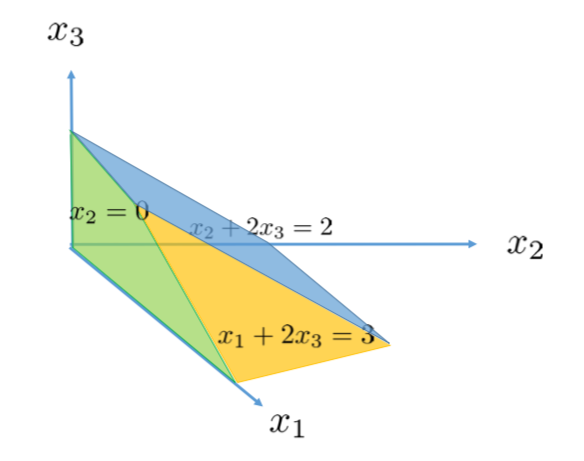
\includegraphics[width=0.5\textwidth]{Second_lecture/p_1}
\caption{Illustration for polyhedral geometry}
\label{fig:2:1}
\end{figure}

Let's introduce some terminologies formally:
\begin{definition}
\begin{itemize}
\item
\emph{Hyperplane} is the set $\{\bm x\mid \bm a\trans\bm x=\bm b\}$
\item
\emph{Half-space} is the set $\{\bm x\mid\bm a\trans\bm x\le\bm b\}$
\item
The \emph{polyhedron} $P$ is the intersection of \emph{finite} number of half-spaces:
\[
P=\left\{
\bm x\middle|
\bm a_i\trans \bm x\le \bm b_i,
\ i=1,\dots,m
\right\}
\]
\item
The \emph{dimension of a polyhedron} is defined as the \emph{lowest} dimension \emph{affine space} containing $P$
\item
The \emph{face} of a polyhedron is defined as
\[
\{\bm x\mid \bm a\trans\bm x=\bm b\}\cap P,
\]
where $P\subseteq\{\bm x\mid \bm a\trans\bm x\le\bm b\}$.
\item
Note that the face of a polyhedron is also a polyhedron. Therefore we define \emph{facet} is the face of $P$ that is one dimensional lower than that of $P$; the \emph{vertex} of $P$ is the face of $P$ that has dimension $0$.
\end{itemize}
\end{definition}
\begin{remark}
In space $\mathbb{R}^n$, normally $n$ hyperplanes intersect at one point
\item
If $P$ is full dimensional (i.e., with diemension $n$), then a vertex of $P$ is an intersection of $n$ facets.
\item
However, sometimes there is a case that more than $n$ hyperplanes intersect at one point, say a vertex, which creates \emph{degeneracy} (show in Fig~(\ref{fig:2:2})).
In such case, adding regularization, i.e., perturbation dimishes over-determination.
\end{remark}
\begin{figure}
\centering
\begin{minipage}[t]{0.48\textwidth}
\centering
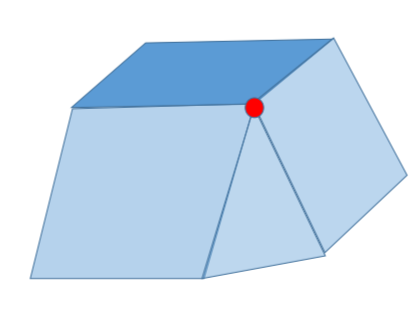
\includegraphics[width=1\textwidth]{Second_lecture/p_2}
\caption{Over-determination results in Degeneracy}
\label{fig:2:2}
\end{minipage}
\begin{minipage}[t]{0.48\textwidth}
\centering
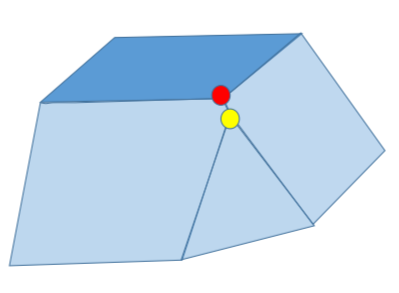
\includegraphics[width=1\textwidth]{Second_lecture/p_3}
\caption{Perturbation diminishes over-determination}
\label{fig:2:3}
\end{minipage}
\end{figure}

\begin{definition}
Given a full dimensional $P$, we say two distinct vertices of $P$ are \emph{adjacent} if they are in the same $n-1$ hyperplane.
\end{definition}
\begin{remark}
Every update for simplex pivots move from a vertice to one of its adjacent position.
\end{remark}
\begin{figure}
\centering
\begin{minipage}[t]{0.48\textwidth}
\centering
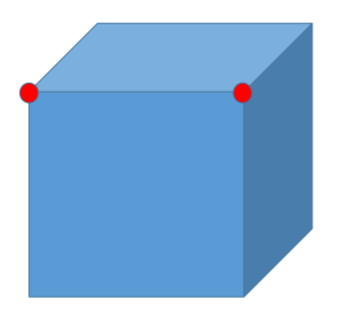
\includegraphics[width=1\textwidth]{Second_lecture/p_4}
\caption{Illustration for \emph{adjacent} vertices}
\label{fig:2:2}
\end{minipage}
\begin{minipage}[t]{0.48\textwidth}
\centering
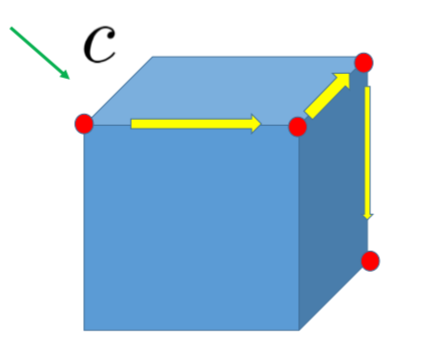
\includegraphics[width=1\textwidth]{Second_lecture/p_5}
\caption{Path for simplex pivots}
\label{fig:2:3}
\end{minipage}
\end{figure}



















